\chapter{Design}
\label{sec:design}
In this chapter, we will discuss the design of our system SPML. Our system SPML aims to protect the confidentiality, integrity, and privacy of the machine learning data and model so that native users don't have to change much of their existing system and yet can achieve stronger privacy and security guarantees. The system consists of two main parts, privacy which is fulfilled using differential privacy, and security which is fulfilled using Trusted Execution Environments (TEEs) for example Intel SGX, ARM TrustZone, etc. In this chapter, the detailed design of the proposed system SPML is described and how each component in the system is achieving our design goals. 
\section{Design Overview}
This section consists of design goals for our system SPML, threat models we are considering, and high-level design for it.
\subsection{Design goal}
All or most of the machine learning models are trained using private and sensitive user data. When such models are used in untrusted environments such as public cloud then privacy, as well as security is always the concern. The goal of any new system is to enable compatibility and usability with early versions so that the existing system can easily be upgraded and adapt to the new features. Keeping all such things under consideration SPML will be designed with the following design goals:
\begin{itemize}
  \item \textbf{Security}: The security means confidentiality and integrity of the data should be protected. To enable security property in SPML, Trusted Execution Environment (TEEs) are used. TEEs protects the application code, model and its parameters, and data inside an enclave and this isolation helps us to achieve our confidentiality and integrity goals.
  \vspace{-0.3cm}\item \textbf{Privacy}: An adversary can still fire many malicious queries on the dataset or trained model to retrieve information of an individual and can breach their privacy. SPML implements differential privacy techniques to preserve privacy.
  \vspace{-0.3cm}\item \textbf{Transparency}: System should be easy to access and use with minimum or no code changes hence APIs should be exposed for the usage of the system so that existing system or code can be upgraded or new features can be integrated easily. SPML uses the SCONE runtime environment which hides the complexity of using TEEs by providing a container-based platform to run any native application with Intel SGX. Additionally, SPML provides easy APIs and any existing system can make use of these APIs with very little code change.
  \vspace{-0.3cm}\item \textbf{Scalability}: It must be easy to scale up the resources of the system. This is one main feature of cloud these days wherein resources can be expanded or contracted easily depending upon the demand from the end-users. SPML being a containerized application support this functionality by default.
  \vspace{-0.3cm}\item \textbf{Performance}: Performance should be the same as the native performance with as little overhead as possible. SPML uses the most promising approach TEEs and start-of-the-art technique differential privacy to achieve security and privacy goals respectively. These approaches or techniques are currently the most optimized one in terms of performance and evolving continuously. Hence, any improvement in these areas will also help our system SPML to further improve its existing performance in the future also.
  \vspace{-0.3cm}\item \textbf{Accuracy}: Accuracy should not change much by enabling security and privacy property. SPML is tested against the hello world dataset of machine learning, MNIST \cite{12}, and CIFAR10 \cite{13} to ensure this.
\end{itemize} 
\subsection{Threat Model}
The goal here is to protect against an attacker in an untrusted environment infrastructure such as public clouds. In the cloud, most of the resources are offered via virtualization either in the form of VMs or containers. If an attacker can intrude in the system it can get hold of all the system resources such as OS, hypervisor, and can attack the system by doing memory dumps. In such a scenario application (code, data, model, and computations) confidentiality, integrity, freshness, and privacy must be preserved. Users can be trusted most of the times but sometimes an adversary might attack the system through inversion attacks i.e black-box queries which might leak data or model. Three types of attacks that can be used to learn an individual's data or model are explained in the background section ~\ref{sec:attackOnML}. We build our system SPML which will be robust and will provide protection against these types of attacks.

Side-channel attacks are not considered as part of this thesis. This is already an active research area. Secondly, it is assumed that the attacker is not able to gain access to the system physically and can enter the processor area to steal secrets or corrupt CPU. Lastly, denial of service attacks are not in scope as the cloud is controlled by a third party operator hence these are not important.


\subsection{High Level Design}
In this section, we will discuss about SPML system overview and its high-level design. To achieve the design goals for SPML, we have design our system using three main components differential privacy, training computation, and inference computation.
\begin{figure}
    \centering
    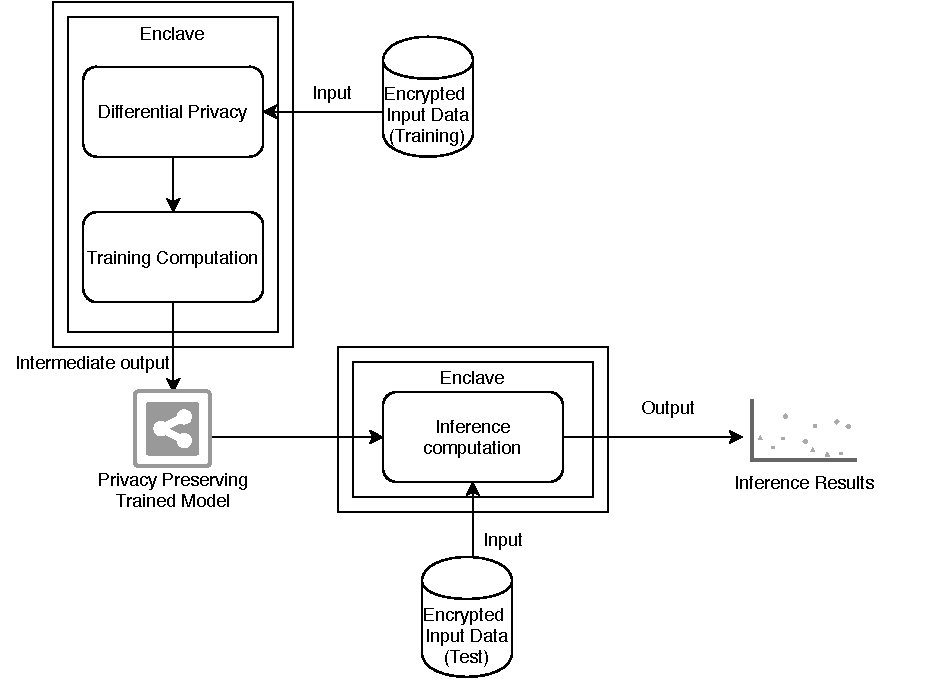
\includegraphics[width=10cm, height=10cm]{images/HLD.pdf}
    \caption{ High-level design}
    \label{fig:hld}
\end{figure}

\begin{itemize}
    \item \textbf{Differential privacy}
This module contains a mechanism to make the input training data differentially private to provide privacy on an individual's data. There are many perturbations techniques available to achieve differential privacy such as input, output, objective, and gradient perturbations. The perturbation techniques works by adding calibrated randomization over the input data before, during, or after the training. The randomization can be achieved using a randomized response technique or adding random noise from Laplace or Gaussian distribution. These noises are added in a way such that computations can be correctly performed and privacy of the data is also preserved \cite{3}. With this module, we will be enabling privacy property in our system SPML. To enable security property, SPML runs this module inside TEEs, which is Intel SGX in our case. 
    \vspace{-0.3cm}\item \textbf{Training computation}
This module is the main training computation module for training the model using the input dataset. The training can be either using machine learning or deep learning mechanisms. It is kind of a wrapper that can be called using APIs without changing much of the existing native machine learning code. This provides transparency and easy use of features for our SPML system. The training of the model takes place inside TEEs to prevent leakage of the trained model.
    \vspace{-0.3cm}\item \textbf{Inference computation}
 The real-world data on which inference is to be performed is kept in an encrypted form on the filesystem to protect its confidentiality and integrity. The user uploads the encrypted data and privacy-preserving trained model (i.e intermediate output of the training phase) in an untrusted environment and activates the inference computation module. The inference computation module performs computation to predict/classify the target output. All these computations take place inside TEEs protecting all the components always. The output of the inference is also saved in an encrypted form to prevent any kind of leakage.
\end{itemize}

Figure ~\ref{fig:hld} shows the high-level design of the SPML system. The workflow begins by uploading an encrypted training dataset to an untrusted enclave enabled cloud. SCONE runtime environment transparently decrypts the input dataset and bring this inside the enclave. The differential privacy module guarantees privacy via noise or randomized response. Depending upon the chosen DP technique corresponding DP module is activated. SPML system then starts training the model using the training computation module. This training can be either using machine learning or deep learning techniques. Both the differential privacy and training computation takes place inside an enclave hence their confidentiality and integrity of these modules are always protected. Training computation will produce a privacy-preserving trained model that will also be encrypted when outside the enclave. This marks the end of the training phase. The inference computation begins when some predictions/classification is to be done on real-word data using this trained model. The inference result will also be saved in an encrypted form when outside the enclave to protect its confidentiality and integrity.

\section{Design Detail}
In this section, the SPML design is explained in detail. The design is split into two phases (1) Training phase and (2) Inference phase. In both of these phases the computation happens inside the TEEs with the help of SCONE.
\begin{figure}
    \centering
    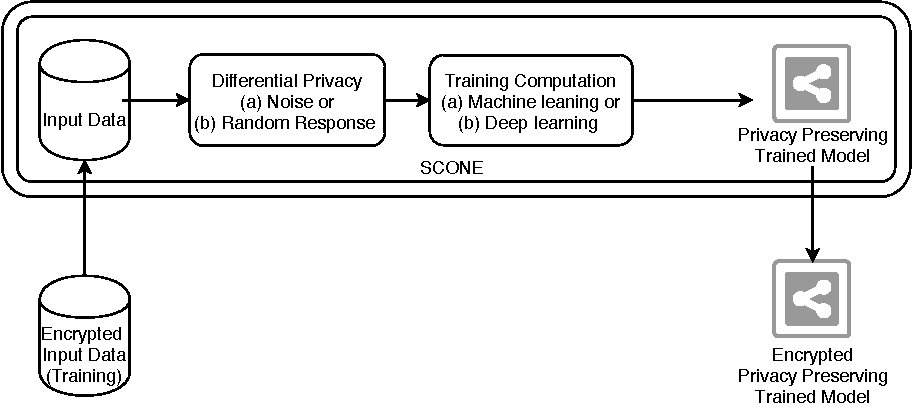
\includegraphics[width=\linewidth]{images/Training.pdf}
    \caption{Training phase}
    \label{fig:trainingDesign}
\end{figure}
\subsection{SCONE}
SCONE \cite{22} provides a platform that can help to build and securely run applications with any TEEs. TEEs provides confidentiality and integrity to the code and data by providing a secure execution region called as an enclave. Together with SCONE and TEEs data, model and code can be protected always. SCONE makes it achievable with minimum effort as there is no need to modify native existing application code. It means encryption/decryption required to protect data and code can be taken care of by SCONE. The secret keys required for encryption/decryption are supplied with the help of SCONE. SCONE has SCONE CAS(configuration and attestation service), which provides policy management and service attestation. The key generation is done inside TEE by SCONE CAS and is managed by a security policy (known as 'Session') of an application. The application code needs not to be changed, the injection of secrets can be done via configuration files or source files or compiled binaries on the TEE which is executing the application. Hence for applications, this process is transparent. SCONE not only gives us an efficient way to run applications within TEEs but it also does transparent encryption and decryption of files without changing the existing source code. SPML uses SCONE as a wrapper over the underlying TEEs (i.e Intel SGX in our case) for achieving confidentiality and integrity in the system.

\subsection{Training phase}
The training phase of our system SPML mainly focuses on training the model. The training is done with the help of the SCONE platform which provides execution in an encrypted manner. This means that data as well as the code are always in encrypted form. Clear text training data and code is only available to the application code. SCONE helps to simplify the encryption of an input, execution of application within the encrypted memory, and encryption of the output. Therefore, SCONE provides end to end transparent encryption/decryption by keeping data in always encrypted form during transmission, rest as well as processing. As shown in Figure ~\ref{fig:trainingDesign}, the input data is kept in an encrypted form on filesystem or harddisk. When computation needs to be performed the encrypted data is brought into the SCONE runtime environment which decrypts it and only application code which is SPML system modules can access that. This way the input data confidentiality and integrity are always protected.  Once the input dataset is decrypted, the privacy property is enabled by calling the differential privacy module.

\subsubsection{Differential privacy}
Differential privacy provides privacy to our system SPML. After choosing the technique of differential privacy that is randomized response or noise the next step is to make input data and model differentially private. If the randomized response is chosen which is our contribution to the SPML system, then the input dataset is made differentially private before training the model. The input dataset (full or some sensitive columns) is randomized using the probability bias p and q, where p is for the first coin flip, and q is for the second flip. The probability bias is the probability of getting the head \cite{14}. 

If noise is chosen then the input is submitted to the trained model and noise is added during the training of the model. For noise, the input dataset itself is not made differentially private but instead, noise is added during the training process in the objective or gradient functions. The noise here means a special type of calibrated random noise based on Gaussian or Laplace distribution. One needs to decide how much noise should be added so that the utility of the trained model is not degraded. If more noise is added then data becomes unusable hence there is always a trade-off between accuracy and utility. This notion is captured using the privacy budget concept as discussed below.

\textbf{Privacy Budget}
Differential privacy works by adding some noise at different levels of points such as before training on the data, during training on the model, or after training at the output. However, more noise means lesser accuracy hence there is always a trade-off to make between noise and accuracy level. This trade-off is defined in the form of mathematical calculation and is termed as $\epsilon$. Differential privacy calculates the privacy loss using this epsilon. There are different ways to calculate privacy loss depending upon the techniques used as follows:
\begin{itemize}
\item \textbf{Random response}
The randomized response works on a mechanism of a coin flip where the first coin is flipped with probability p and the second coin is flipped with probability q. These p and q are called bias, which are the probabilities of getting head. It provides $\epsilon$-\text{differential privacy}. To calculate epsilon and privacy loss for a randomized response, equations suggested in \cite{18} are used :
\begin{equation}
\epsilon = \log({\frac{p + (1 - p) * q}{(1 - p) * q}})
\label{eq:epsRR}
\end{equation}
Equation ~\ref{eq:epsRR} is used to calculate the epsilon value. For different p and q values, epsilon value differs and hence p and q can be used to control how much privacy or noise should be added.
\item \textbf{Noise}
Noise is added based on Gaussian Distribution or Laplace Distribution. Laplace satisfies $\epsilon$-\text{differential privacy} while Gaussian satisfies ($\epsilon$,$\delta$)-\text{differential privacy}. In our system SPML, we have used Gaussian noise and to calculate ($\epsilon$,$\delta$)-\text{differential privacy} the current method as discussed in equation ~\ref{eq:epsGaussian} is not an accurate fit, especially when composition with heterogeneous mechanisms is involved \cite{4} as in our system SPML. We will be using Rényi divergence to measure differential privacy based on paper \cite{23} which provides Rényi Differential Privacy (RDP), instead of using differential privacy in equation ~\ref{eq:epsGaussian}. SPML uses sampling distribution along with Gaussian noise and RDP is a perfect fit to calculate privacy when sampling is involved.
\end{itemize}
\subsubsection{Training Computation}
This is the module where the main machine learning computation happens. There are a lot of machine learning frameworks available to develop and train models such as Pytorch \cite{75}, Tensorflow \cite{24}, Scikit-learn library \cite{62}, etc. Depending upon the type of problem under consideration either machine learning or deep learning technique can be used. To train the differentially private model simple APIs are used like in the existing native machine learning/deep learning system with optimizers and loss functions. This computation takes place inside the SCONE and hence is secured even from the root user.

The training phase will produce a secure privacy-preserving trained model as shown in Figure ~\ref{fig:trainingDesign}. This model will not only protects confidentiality and integrity but also the privacy of the individuals. SCONE runtime environments encrypt this model before saving it to the filesystem. The encrypted trained model is used for inference by uploading it to the trusted environment when needed. The size of the model is usually small and hence it is easily portable and can be scaled up and down depending upon the demand providing easy portability and scalability. 
\begin{figure}
    \centering
    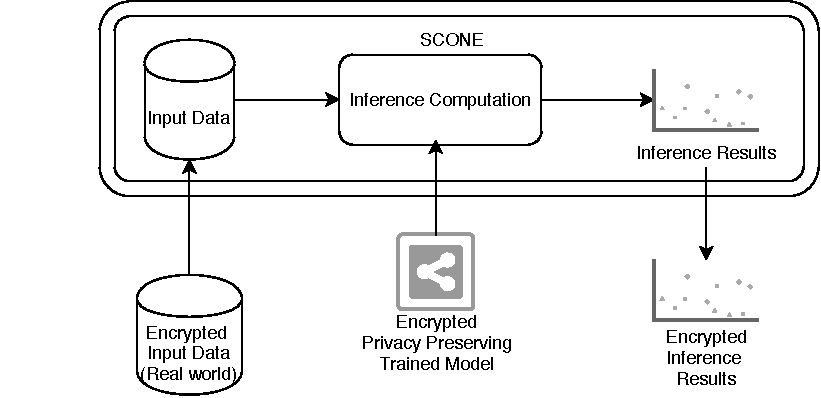
\includegraphics[width=\linewidth]{images/Inference.pdf}
    \caption{Inference phase}
    \label{fig:inferenceDesign}
\end{figure}
\subsection{Inference phase}
The inference phase of our system SPML means predicting/classifying on the trained model obtained from the last phase. The real-world data against which prediction/classification is to be made is also kept in an encrypted form in a filesystem. SCONE runtime environment is responsible for transparently decrypt it and provide clear text real-world data inside the enclave for inference. The real-world data is data that is not known to the previously trained model. This is the actual data of interest on which inference is required. As shown in Figure ~\ref{fig:inferenceDesign}, the input real-world data on which inference is to be made is fed into the inference computation module along with the trained model. This computation takes place inside the enclave, which means all the computation, model, and data are kept always encrypted in an untrusted environment. Inference computation involves correlating input data to predict/classify the output and coughing out the best possible outcome. \textbf{Encrypted inference result} will be the output of this phase and this is also encrypted by the SCONE runtime environment before saving it to the filesystem. Once, we have got the inference result, it marks the end of our system workflow.

\section{Summary}
Our system SPML provides privacy guarantees using differential privacy techniques to protect an individual's information. The confidentiality and integrity properties are enabled using TEE which in our case is Intel SGX. The SCONE runtime environment provides easy integration with TEEs. SCONE runtime environments take care of transparent encryption and decryption as well as make sure that all the data and computation happens inside the TEE. 

SPML consists of two phases training phase and the inference phase. In the training phase of SPML, we enable privacy property, and the model is trained with this property enabled. The privacy property is achieved using differential privacy and hence the trained model is privacy-preserving. By running SPML with TEEs security property gets enabled by default. With these two properties enabled, we can make any existing native machine learning system a secure privacy-preserving system. In the inference phase of SPML, we use a secure privacy-preserving model(i.e encrypted private model) obtained from the training phase to provide inference on real-world data. In this phase, also security property is enabled by default, hence inference results are always encrypted.

There are no changes required in the existing source code of the application and this helps us to fulfill our transparency goal. SCONE works in a docker like environment hence system can be easily scaled up and down on demand. SPML can be easily deployed in an untrusted enclave enabled cloud environment without the need to change anything. SCONE has very little overhead hence performance and accuracy are not much effected for the overall system. The SPML is designed in a way so that it fulfills all the discussed design goals. In the next chapter, we will discuss how we have implemented our system SPML.

